\documentclass{beamer}
\usecolortheme{orchid}
%\usepackage{graphicx}
\usepackage{hyperref}
\hypersetup{
    colorlinks=true,
    linkcolor=blue,
    filecolor=magenta,      
    urlcolor=cyan,
}
\usepackage[autoplay,loop]{animate} % I stuck the `autoplay' and `loop' functions up here to make it the default.

\title{Embedding ``GIFs'' in Beamer Slides \\ Memes for Fun, Profit, and Embarrassing Your Colleagues}
\author{Alton B.H. Worthington}
\institute{University of Michigan}
\date{5/6 December 2016}

% This block of comment is to 1) Thank folks on Twitter for giving me something better to do on a couple of evenings than work on a dissertation 2) apologize to those who have seen this slide format before at a conference - I only have one style 3) apologize for my crummy code and lame jokes, and 4) disclaim all responsibility for all of that stuff that lawyers talk about at the end of pharmaceutical commercials.

% PS: I release all ownership of this LaTeX code. Use, splice, edit, distribute as you will.



\begin{document}
\beamertemplateshadingbackground{blue!10}{gray!30}
\usenavigationsymbolstemplate{}
\frame{\titlepage}

\begin{frame}
	\frametitle{Motivation}
	Why even bother with GIFs? GIFs are:
		\begin{itemize}
			\item Super Old-school
			\item Space-inefficient (you want 400MB presentations? This is how you get 400MB presentations.)
			\item Not particularly attractive
			\item Actually kind of a pain in the butt to do in \LaTeX
			\item Guaranteed to be mentioned in your tenure file... I assume.
		\end{itemize}
	This seems like a bad idea. Are you sure?
\end{frame}

\begin{frame}
	\begin{center}
	\animategraphics[width=.75\linewidth]{25}{jack/jack-}{0}{82} %this command is: \animategraphics[options]{frames per second}{root of filename}{first frame number}{last frame number} - I knew to use 33.33 fps because I cheated and looked at the GIF properties (30ms per frame) in GIMP. You may choose to eyeball this. This all comes up again in the slides later on down there...
	\end{center}
\end{frame}

\begin{frame}
	\frametitle{I lied to you. That wasn't a GIF. (If you didn't notice already.)}
	Unfortunately, you can't really put a GIF directly into a PDF anymore. One used to be able to cram it into a PDF, open it in Acrobat Reader, then let an outboard player (like Flash Player) do the work. This is no longer an option. This is also, given the concerns on the previous slide, a ``good thing''.
	\begin{block}{I Made a Huge Mistake}
		Since I haven't tried to put a GIF in a slideshow in years, I never realized things had changed before I promised this instructional document. I lied. I'm sorry. Or, blame the PDF standard-setters. Your call.
	\end{block}
	The good news is that you can still ``embed'' a ``GIF'', but there's a bit more legwork to it.
\end{frame}

\begin{frame}
	\frametitle{But I want to make bad career choices!!!!}
	Ok. Suit yourself.
	\begin{figure}
		\centering
		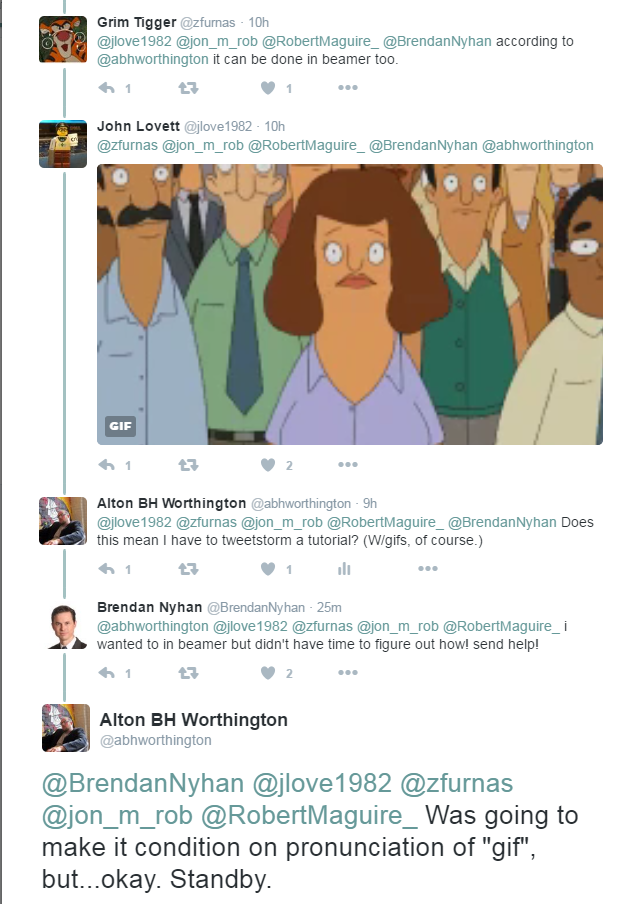
\includegraphics[scale=.25]{genesis.PNG}
	\end{figure}
	We all make mistakes. \pause I mean, I took the time to make a meta-beamer stack. If you're sure about this, proceed.
\end{frame}

\begin{frame}
	\frametitle{Ingredients}
	Congratulations! You've decided to make memetics a pedagogical strategy. Here's what you need:
		\begin{itemize}
			\item A gif. Or gifs.
			\item \href{https://www.imagemagick.org/script/binary-releases.php}{ImageMagick} (it's available for all OSes)
			\item Beamer
			\item A bit of time and a folder to hold everything - your GIF is going to become a series of frames
			\item Optional, but recommended: \href{https://www.roosroast.com/}{coffee}
		\end{itemize}
	This is a beginner's guide, the ``hello world'' version of this process. I'll direct you to more documentation at the end of this stack.
\end{frame}

\begin{frame}
	\frametitle{Step 1a: Acquire the Memes of Production}
	This should be self explanatory. Find a gif you like or which is relevant to your interests. Good candidates include:
		\begin{itemize}
			\item Cats
			\item Movies
			\item Famous people
			\item Relatable cartoons
			\item Internet esoterica
		\end{itemize}
	Shorter GIFs work better for this, but it's not a huge deal.
\end{frame}

\begin{frame}
	\frametitle{Step 1b: Premium GIFs}
	If you can get multiple at once, you're in with a shot at a conference award. (Please share the award money.)
	\begin{center}
	\animategraphics[width=\linewidth]{18}{cat/cat-}{0}{49}
	\end{center}
	\end{frame}

\begin{frame}
	\frametitle{Step 1c: Saving and Organizing}
	Once you've found your premium GIF material:
		\begin{enumerate}
			\item Create a folder somewhere convenient. (read: somewhere with a short filepath)
			\item Save the GIF to that convenient location.
			\item Prepare to break your GIF up.
		\end{enumerate}
\end{frame}

\begin{frame}
	\frametitle{Step 2a: Breaking Up}
	GIFs are great, but they won't work as-is in beamer or in \LaTeX. You could convert it to a movie, but an easier route  is to create images and animate it. You've got a few options:
		\begin{itemize}
			\item Various web services (that's between you and Google)
			\item GIMP or other image editing software
			\item or, my recommendation: \href{https://www.imagemagick.org/script/binary-releases.php}{ImageMagick}
		\end{itemize}
	ImageMagick has a bit of a learning curve, but let's face it: You're using \LaTeX. You've got this.
\end{frame}

\begin{frame}
	\frametitle{Step 2b: Download and Install ImageMagick}
	I use \href{https://www.imagemagick.org/script/binary-releases.php}{ImageMagick} to convert a GIF into individual images. It does \emph{a whole lot more}, but for today, we are just going to use it to convert the GIF into a stack of PNG images, which pdflatex finds easy to digest. First you have to download and install it! \\
	Once you've installed it, you operate it from a command line. The instructions give you a first walkthrough, but as a reminder:
		\begin{itemize}
			\item In Windows, go to the start menu and run ``cmd.exe''
			\item In OSX, go to Applications $\rightarrow$ Utilities (or Spotlight) and launch terminal.
			\item If you are using any Linux/Unix, I trust you know what to do.
		\end{itemize}
	The next step is the only bit of command line messiness you need to deal with. Sorry. It's worth it, I promise.
\end{frame}

\begin{frame}
	\frametitle{Step 2c: From GIF to PNG}
	
	
\end{frame}


\begin{frame}
	\frametitle{Step 3a: Animating in Beamer - Roll-your-own GIFs}
	
\end{frame}



\begin{frame}
	\frametitle{If all has gone well, you'll look at your presentations like:}
	\begin{center}
	\animategraphics[width=\linewidth]{20}{comp/comp-}{0}{223}
	\end{center}
\end{frame}

\begin{frame}
	\frametitle{Your presentations are gonna be so great, your audience will:}
	\begin{center}
	\animategraphics[width=\linewidth]{12.5}{lakerbros/lakerbros-}{0}{42}
	\end{center}
\end{frame}

\begin{frame}
	\frametitle{Or, better yet:}
	\begin{center}
	\animategraphics[width=\linewidth]{12.5}{lakerbros/lakerbros-}{42}{0}
	\end{center}
	\pause
(Those are the same files, btw. Just reversed the frame order. It's fun.)
\end{frame}

\begin{frame}
	\frametitle{References/Additional Info}
	
\end{frame}

\begin{frame}
	\frametitle{Thanks to:}
	\begin{itemize}
		\item 
	\end{itemize}
\end{frame}

\end{document}